\section{Testing plan}

The main goals of this performance testing plan are:
\begin{itemize}
  \item to find out whether the usage of LSM implies some sort of performance penalty;
  \item to identify possible improvable points when embedding WebAssembly in another language.
\end{itemize}

\noindent
For a given program, the following different builds are tested:
\begin{itemize}
  \item the native binary, obtained through \texttt{rustc}, run directly;
  \item the native binary run with Landlock and through eBPF;
  \item the WebAssembly binary run directly by \textit{Wasmtime};
  \item the WebAssembly binary run by the developed program with Landlock enabled and disabled;
  \item the WebAssembly binary run through eBPF (using \textit{Wasmtime}).
\end{itemize}

All programs are compiled with optimisations enabled for both a native binary and a WebAssembly binary.

\subsection{System and hardware}

The system and hardware used for both the development of the project described in Section \ref{sec:restricting-wasi-landlock}
and the performed test is as follows:
\begin{itemize}
  \item Arch Linux as the operating system, more specifically the 2022.05.01 version;
  \item an Intel Core i5-7200U quad-core with a clock rate of 2.5 GHz;
  \item 8 GB of RAM;
  \item a 120 GB solid state disk.
\end{itemize}

The choice of the operating system is mainly dictated by the fact that Arch Linux has both Landlock and eBPF active
out of the box, removing the need to compile the Linux kernel with the necessary flags to enable these
functionalities.

\subsection{Tests' description}

The performed tests are:
\begin{itemize}
  \item a purely computational program, given by the sorting of 10000 random numbers as in Listing \ref{lst:sorting-test-rust},
        in order to measure the pure computational impact of the various methods;
  \item a simple reading of files of various sizes as in Listing \ref{lst:reading-test-rust}, with only the necessary permissions enabled on
        a case by case bases, in order to test the sandbox provided and how they fare against native binaries.
\end{itemize}

The reading file test is repeated with different file sizes\footnote{Randomly generated by using \texttt{/dev/urandom}.},
which are $100$ KB, $1$ MB, $10$ MB and $100$ MB. By doing this, it is possible to see how performance
varies when dealing with progressively large files.

\vspace*{0.5cm}
\begin{code}[language=Rust, caption=The tested ``sorting program''., label=lst:sorting-test-rust]
use rand::Rng;

fn main() {
  let mut rng = rand::thread_rng();
  let mut vec: Vec<i32> = Vec::new();

  for _ in 0..10000 {
    vec.push(rng.get::<i32>());
  }

  vec.sort();
}
\end{code}

\begin{code}[language=Rust, caption=The tested ``reading program''., label=lst:reading-test-rust]
fn main() {
  let content = std::fs::read("input-file.txt");
  match content {
      Ok(c) => println!("{}", c.len()),
      Err(_e) => std::process::exit(1),
  }
}
\end{code}

\subsection{Performance indicators}

The main performance indicators will be the mean execution time, measured in milliseconds, together with its
standard deviation in order to compensate for variability.
These measures are always obtained from a sample of 100 runs, executed and measured by \texttt{hyperfine},
a command-line benchmarking tools \cite{hyperfine}, and finally saved to a
JSON file.

In this chapter, we define for brevity $\mu_x$ to be the mean of the method $x$ and $\sigma_x$ to be
the standard deviation of the method $x$.

\section{Comparison between different methods}

In this section we will look at what impact different LSMs bring on a program,
be it a native binary or a WebAssembly binary run through some kind of runtime.

\subsection{Landlock and eBPF on a native binary}
\label{sec:landlock-vs-ebpf-native}

As it is visible in Table \ref{table:lsm-impact-native}, when dealing with a purely computational program
Landlock is closer to native speed than eBPF, although the difference is on the order
of 2 ms and so it is essentially negligible.
This is shown also in the three graphs in Figure \ref{fig:distribution-sorting-native} - all runs are
concentrated under 5 ms.

\begin{table}
  \centering
  \csvreader[
    tabular={|l|r|r|r|r|r|r|},
    table head = \hline
      \textit{Test type}
      & $\mu_\mathrm{Native}$   & $\sigma_\mathrm{Native}$
      & $\mu_\mathrm{Landlock}$ & $\sigma_\mathrm{Landlock}$
      & $\mu_\mathrm{eBPF}$     & $\sigma_\mathrm{eBPF}$ \\ \hline\hline,
    late after line = \\ \hline,
    head to column names,
  ]{test-data/native-landlock-ebpf.csv}{}
  {\type & \mnative & \snative & \mlandlock & \slandlock & \mebpf & \sebpf}
  \caption{Execution times of a native binary under different restrictions (in ms).}
  \label{table:lsm-impact-native}
\end{table}

\begin{figure}[ht]
  \centering
  \begin{subfigure}[b]{0.32\textwidth}
    \centering
    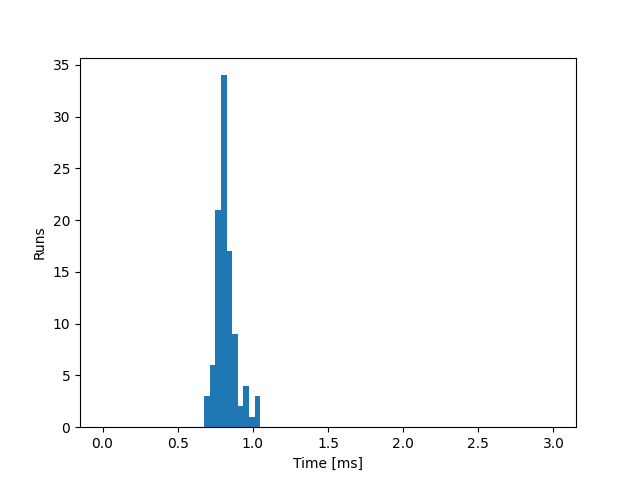
\includegraphics[width=\textwidth]{tests/sorting.native.png}
    \caption{Native}
  \end{subfigure}
  \begin{subfigure}[b]{0.32\textwidth}
    \centering
    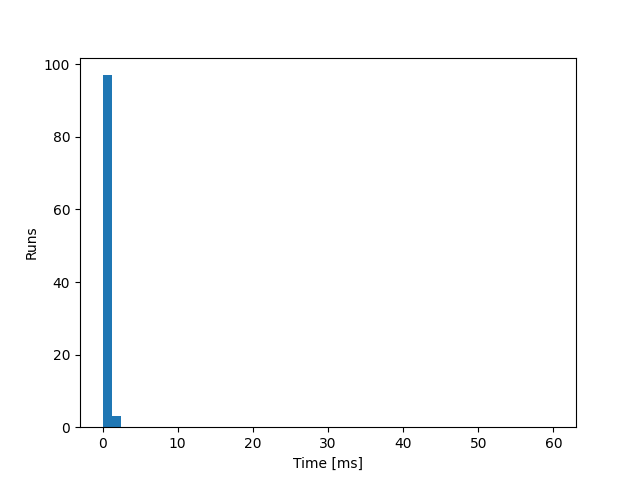
\includegraphics[width=\textwidth]{tests/sorting.native-landlock.png}
    \caption{Landlock}
  \end{subfigure}
  \begin{subfigure}[b]{0.32\textwidth}
    \centering
    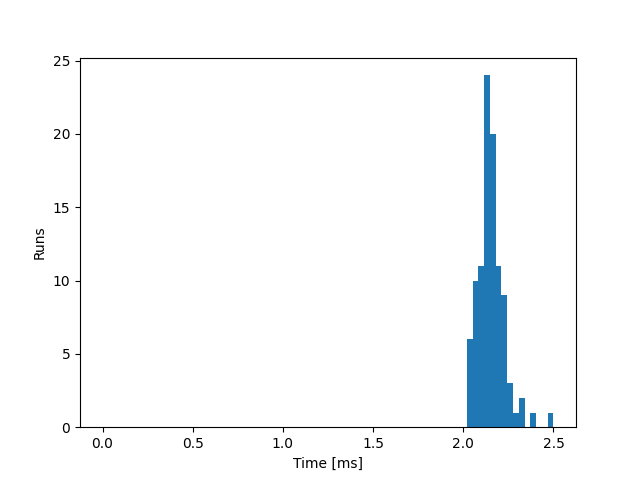
\includegraphics[width=\textwidth]{tests/sorting.bpf.png}
    \caption{eBPF}
  \end{subfigure}
  \caption{Distribution of run times when sorting 10000 numbers (native).}
  \label{fig:distribution-sorting-native}
\end{figure}

Similarly, when dealing with files there the use of LSMs does not bring a great overhead.
Execution times of protected binaries are always comparable to running a binary directly
without any form of restriction. Moreover, as seen in Figure \ref{fig:avg-comparison-native-speed},
the various functions of the average follow more or less the same shape.
Times get significantly higher when dealing with files with sizes in the order of hundreds of MBs,
but even in this case execution times do not differ a lot - restricted binaries however show
lower variability.

Note that in all these tests eBPF performs always worse on average than Landlock - this could be
due to the fact that, when running \texttt{bpfcontain}, there is a communication with an active daemon
(as explained in Section \ref{sec:restricting-wasi-ebpf}), while Landlock communicates directly with
the Linux kernel.

\begin{figure}[h]
  \centering
  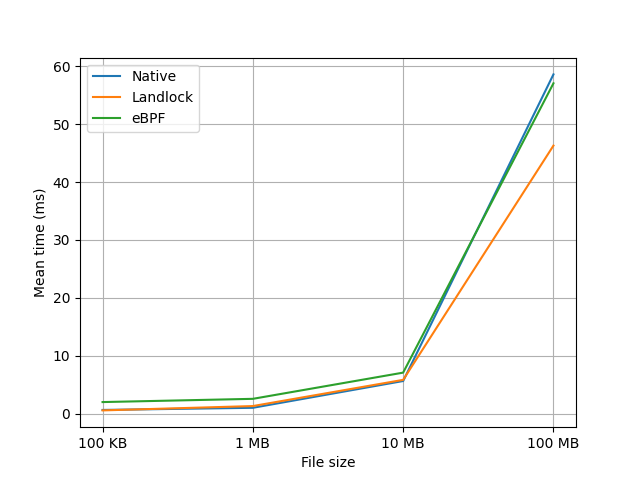
\includegraphics[width=0.8\linewidth]{tests/reading-file-native-graph.png}
  \caption{A comparison of native average speeds when reading a file.}
  \label{fig:avg-comparison-native-speed}
\end{figure}

\begin{figure}[h!]
  \centering
  \begin{subfigure}[b]{0.32\textwidth}
    \centering
    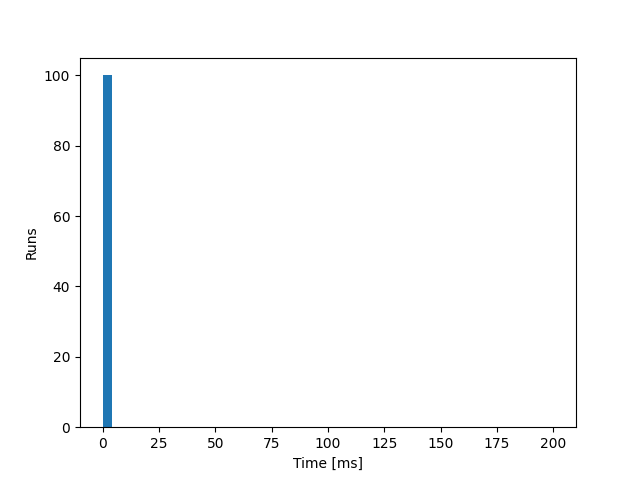
\includegraphics[width=\textwidth]{tests/reading-file-100k.native.png}
    \caption{Native (100 KB)}
  \end{subfigure}
  \begin{subfigure}[b]{0.32\textwidth}
    \centering
    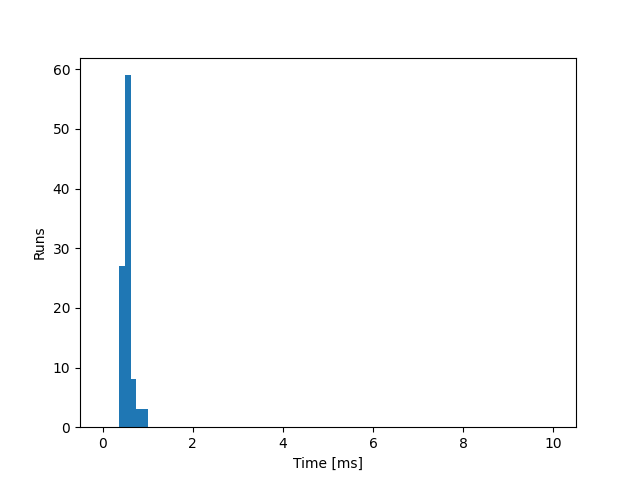
\includegraphics[width=\textwidth]{tests/reading-file-100k.native-landlock.png}
    \caption{Landlock (100 KB)}
  \end{subfigure}
  \begin{subfigure}[b]{0.32\textwidth}
    \centering
    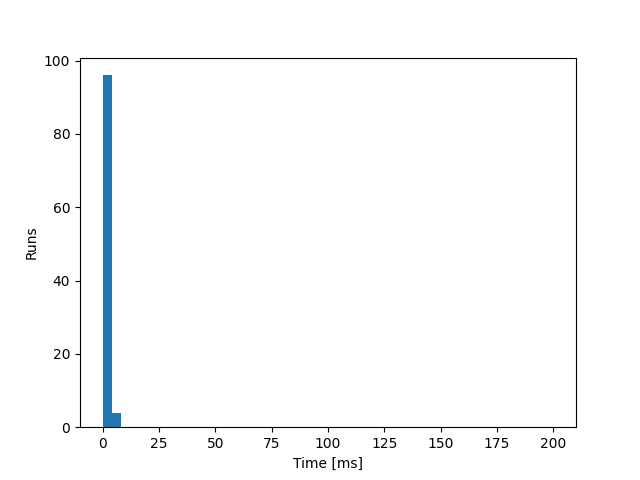
\includegraphics[width=\textwidth]{tests/reading-file-100k.bpf.png}
    \caption{eBPF (100 KB)}
  \end{subfigure}

  \begin{subfigure}[b]{0.32\textwidth}
    \centering
    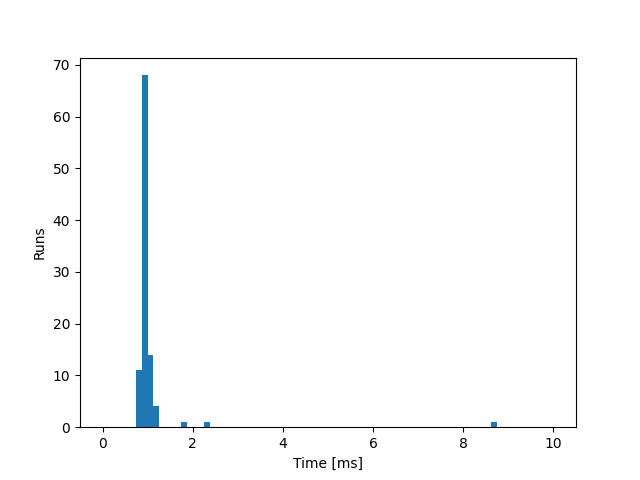
\includegraphics[width=\textwidth]{tests/reading-file-1M.native.png}
    \caption{Native (1 MB)}
  \end{subfigure}
  \begin{subfigure}[b]{0.32\textwidth}
    \centering
    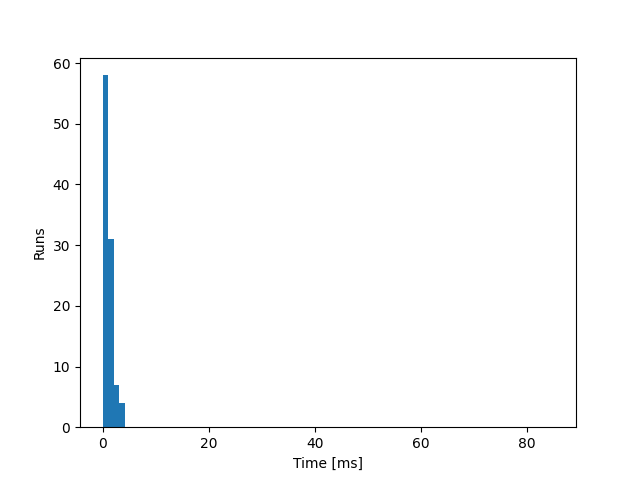
\includegraphics[width=\textwidth]{tests/reading-file-1M.native-landlock.png}
    \caption{Landlock (1 MB)}
  \end{subfigure}
  \begin{subfigure}[b]{0.32\textwidth}
    \centering
    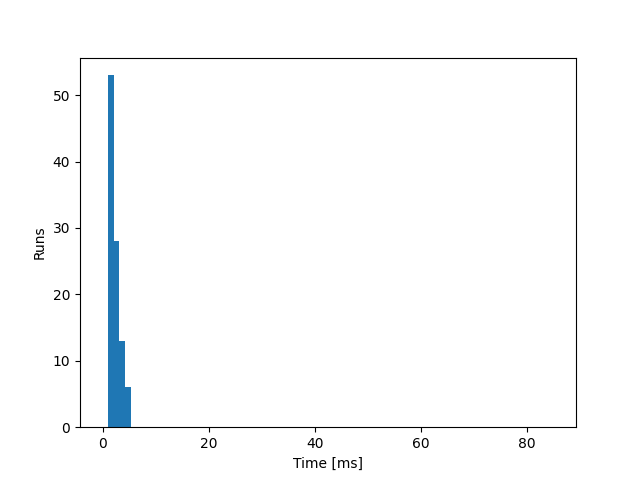
\includegraphics[width=\textwidth]{tests/reading-file-1M.bpf.png}
    \caption{eBPF (1 MB)}
  \end{subfigure}

  \begin{subfigure}[b]{0.32\textwidth}
    \centering
    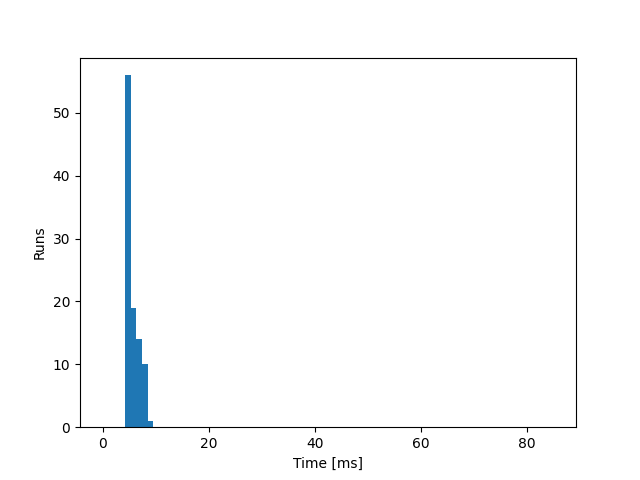
\includegraphics[width=\textwidth]{tests/reading-file-10M.native.png}
    \caption{Native (10 MB)}
  \end{subfigure}
  \begin{subfigure}[b]{0.32\textwidth}
    \centering
    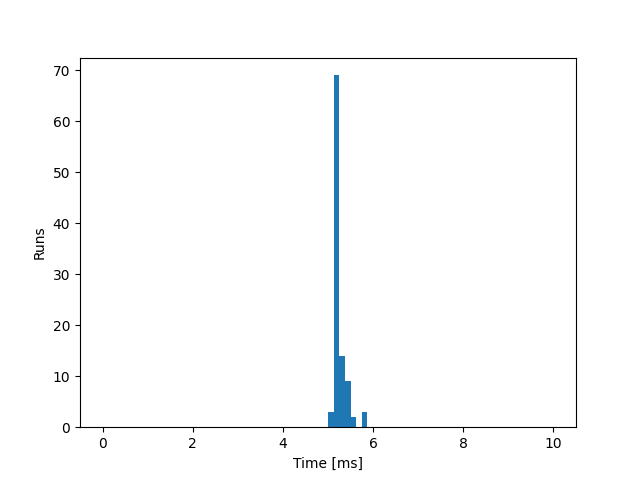
\includegraphics[width=\textwidth]{tests/reading-file-10M.native-landlock.png}
    \caption{Landlock (10 MB)}
  \end{subfigure}
  \begin{subfigure}[b]{0.32\textwidth}
    \centering
    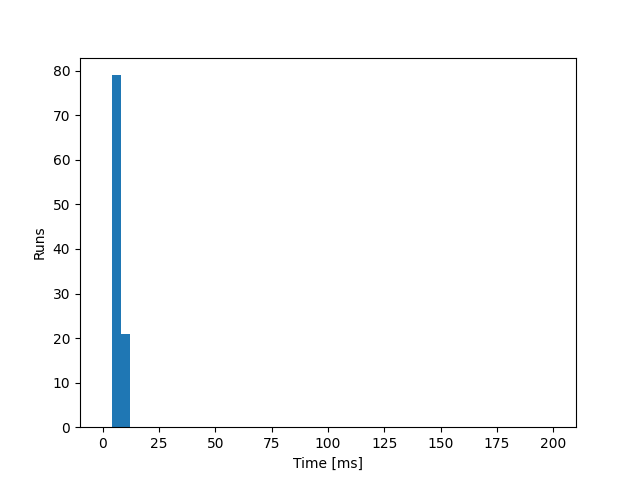
\includegraphics[width=\textwidth]{tests/reading-file-10M.bpf.png}
    \caption{eBPF (10 MB)}
  \end{subfigure}

  \begin{subfigure}[b]{0.32\textwidth}
    \centering
    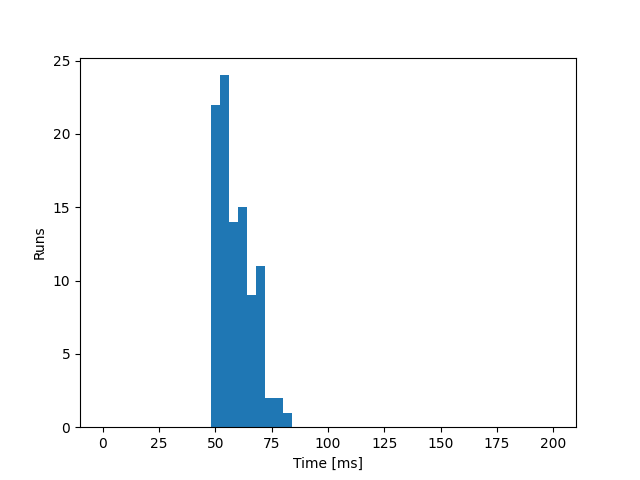
\includegraphics[width=\textwidth]{tests/reading-file-100M.native.png}
    \caption{Native (100 MB)}
  \end{subfigure}
  \begin{subfigure}[b]{0.32\textwidth}
    \centering
    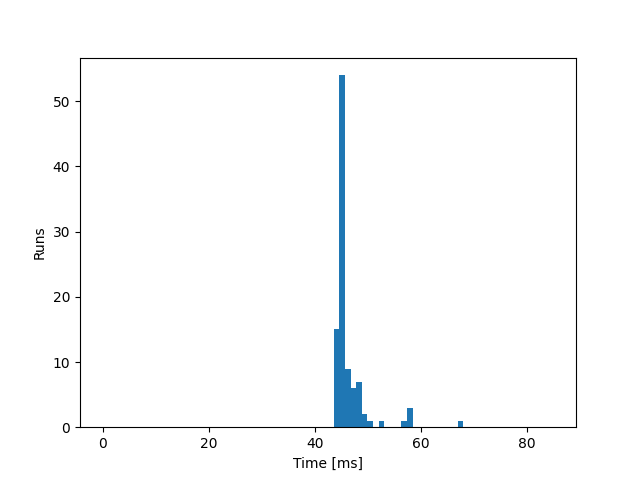
\includegraphics[width=\textwidth]{tests/reading-file-100M.native-landlock.png}
    \caption{Landlock (100 MB)}
  \end{subfigure}
  \begin{subfigure}[b]{0.32\textwidth}
    \centering
    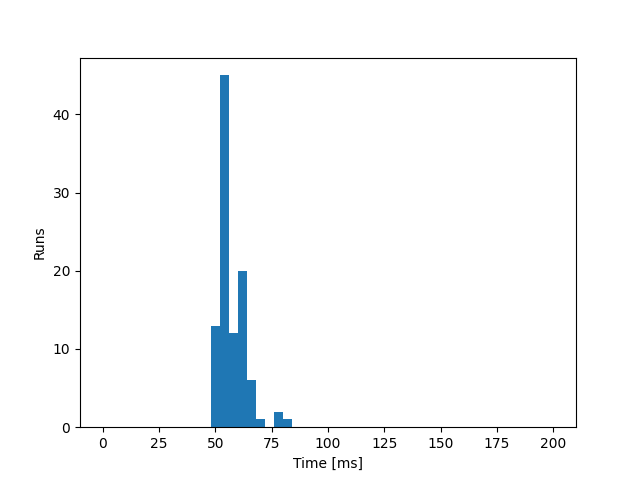
\includegraphics[width=\textwidth]{tests/reading-file-100M.bpf.png}
    \caption{eBPF (100 MB)}
  \end{subfigure}

  \caption{Distribution of a native binary execution times when reading a file.}
  \label{fig:distribution-reading-native}
\end{figure}


\subsection{Landlock and eBPF on a WebAssembly binary}

The first thing of note, immediately shown by the data in Table \ref{table:lsm-impact-wasm},
is that on average every single execution of a WASM binary, either restricted or not,
is slower than running directly a native binary. This is also shown in the three distribution
graphs visible in Figure \ref{fig:distribution-sorting-wasm}, especially when compared with
the ones in Figure \ref{fig:distribution-sorting-native}.

Hence, a WASM binary performance is reasonably comparable to a native binary,
although there is a constant overhead of at least 20 ms in all the test runs.

\begin{table}
  \centering
  \csvreader[
    tabular={|l|r|r|r|r|r|r|},
    table head = \hline
      \textit{Test type}
      & $\mu_\mathrm{Wasmtime}$   & $\sigma_\mathrm{Wasmtime}$
      & $\mu_\mathrm{Landlock}$ & $\sigma_\mathrm{Landlock}$
      & $\mu_\mathrm{eBPF}$     & $\sigma_\mathrm{eBPF}$ \\ \hline\hline,
    late after line = \\ \hline,
    head to column names,
  ]{test-data/wasm-landlock-ebpf.csv}{}
  {\type & \mnative & \snative & \mlandlock & \slandlock & \mebpf & \sebpf}
  \caption{Execution times of a WASM binary under different restrictions (in ms).}
  \label{table:lsm-impact-wasm}
\end{table}

\begin{figure}[ht]
  \centering
  \begin{subfigure}[b]{0.32\textwidth}
    \centering
    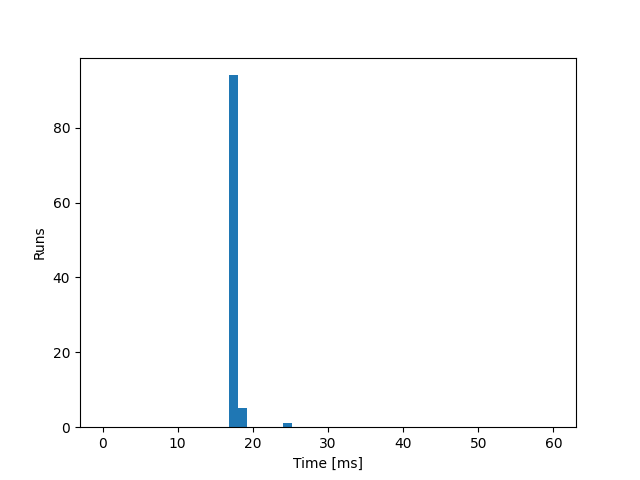
\includegraphics[width=\textwidth]{tests/sorting.wasmtime.png}
    \caption{Wasmtime}
  \end{subfigure}
  \begin{subfigure}[b]{0.32\textwidth}
    \centering
    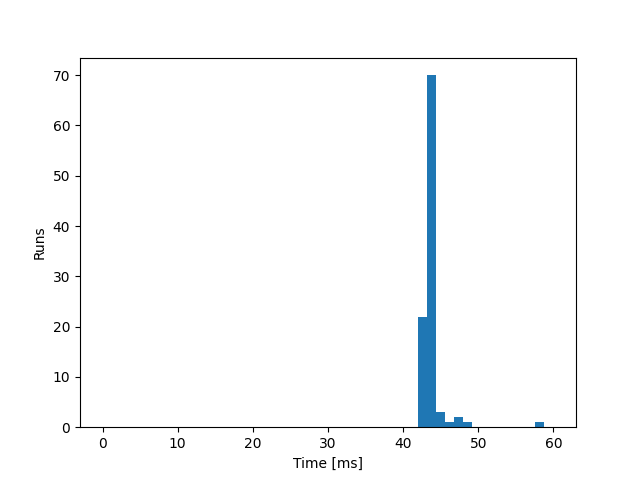
\includegraphics[width=\textwidth]{tests/sorting.landlock.png}
    \caption{Wasmtime + Landlock}
  \end{subfigure}
  \begin{subfigure}[b]{0.32\textwidth}
    \centering
    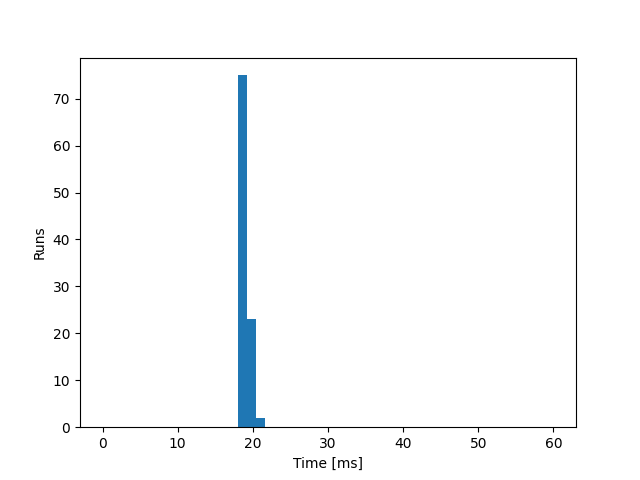
\includegraphics[width=\textwidth]{tests/sorting.bpf-wasmtime.png}
    \caption{Wasmtime + eBPF}
  \end{subfigure}
  \caption{Distribution of execution times when sorting 10000 numbers (WASM).}
  \label{fig:distribution-sorting-wasm}
\end{figure}

There is another interesting result that presents itself when analysing the integration of Landlock
and the embedding of WebAssembly modules in Rust (through \textit{Wasmtime}) -
a constant overhead with respect to using \textit{Wasmtime} directly or through eBPF.
This can be seen in Table \ref{table:lsm-impact-wasm}, but is more visible in Figure \ref{fig:avg-comparison-wasm-speed},
showing how the average execution time varies with respect to read file size -
the \textit{Landlock} curve has roughly the same shape as the other two, but appears translated
of a constant factor of around 30 ms.

Since in Section \ref{sec:landlock-vs-ebpf-native} it was shown that no restriction method had a considerable overhead
against a native binary, and because in this case the WASM module is interpreted by a native binary
restricted with Landlock, it stands to reason that this overhead should be due to the usage
of the library provided by \textit{Wasmtime} for integrating WASM in Rust.

In all cases, however, execution times are not higher than 200 ms - although being a noticeable
delay, this is small enough to not be of any discomfort to a human user.

\begin{figure}[h!]
  \centering
  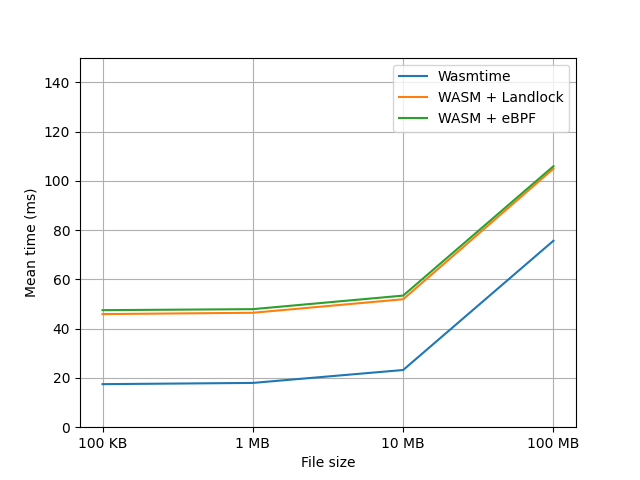
\includegraphics[width=0.8\linewidth]{tests/reading-file-wasm-graph.png}
  \caption{A comparison of WASM average speeds when reading a file.}
  \label{fig:avg-comparison-wasm-speed}
\end{figure}

\begin{figure}[h!]
  \centering
  \begin{subfigure}[b]{0.32\textwidth}
    \centering
    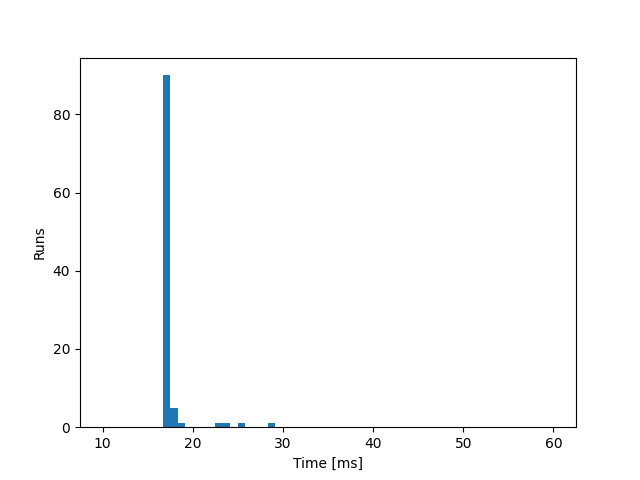
\includegraphics[width=\textwidth]{tests/reading-file-100k.wasmtime.png}
    \caption{Wasmtime (100 KB)}
  \end{subfigure}
  \begin{subfigure}[b]{0.32\textwidth}
    \centering
    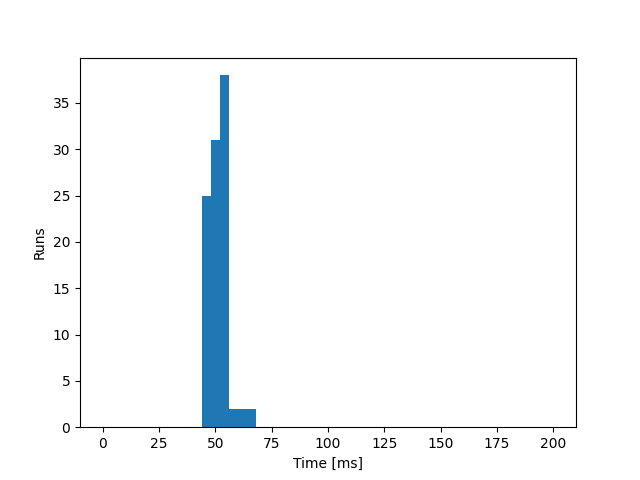
\includegraphics[width=\textwidth]{tests/reading-file-100k.landlock.png}
    \caption{Landlock (100 KB)}
  \end{subfigure}
  \begin{subfigure}[b]{0.32\textwidth}
    \centering
    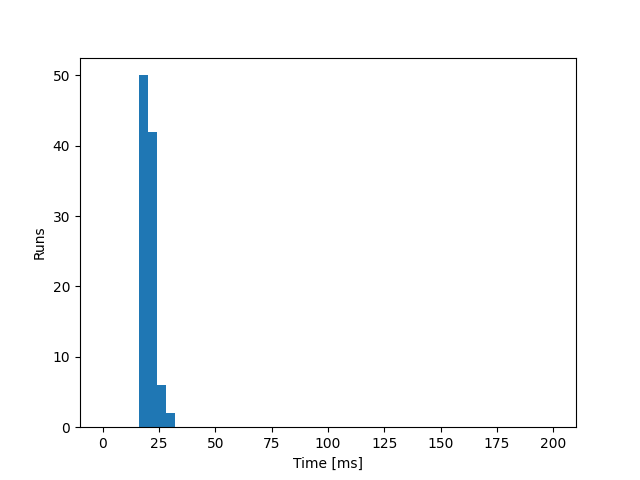
\includegraphics[width=\textwidth]{tests/reading-file-100k.bpf-wasmtime.png}
    \caption{eBPF (100 KB)}
  \end{subfigure}

  \begin{subfigure}[b]{0.32\textwidth}
    \centering
    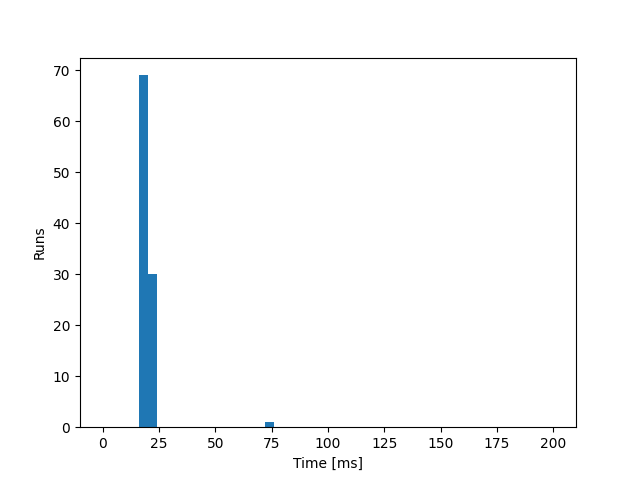
\includegraphics[width=\textwidth]{tests/reading-file-1M.wasmtime.png}
    \caption{Wasmtime (1 MB)}
  \end{subfigure}
  \begin{subfigure}[b]{0.32\textwidth}
    \centering
    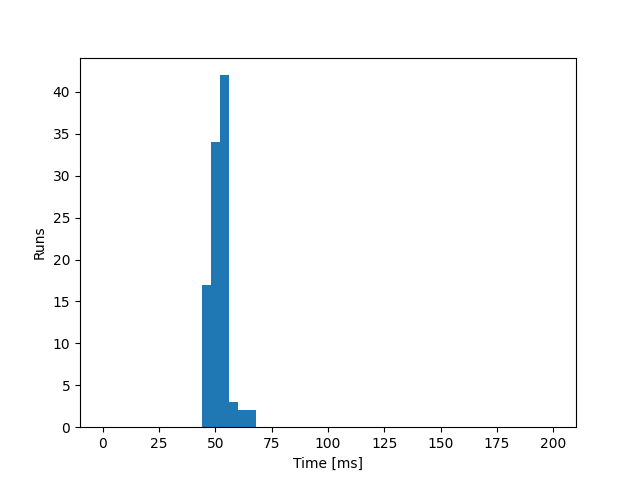
\includegraphics[width=\textwidth]{tests/reading-file-1M.landlock.png}
    \caption{Landlock (1 MB)}
  \end{subfigure}
  \begin{subfigure}[b]{0.32\textwidth}
    \centering
    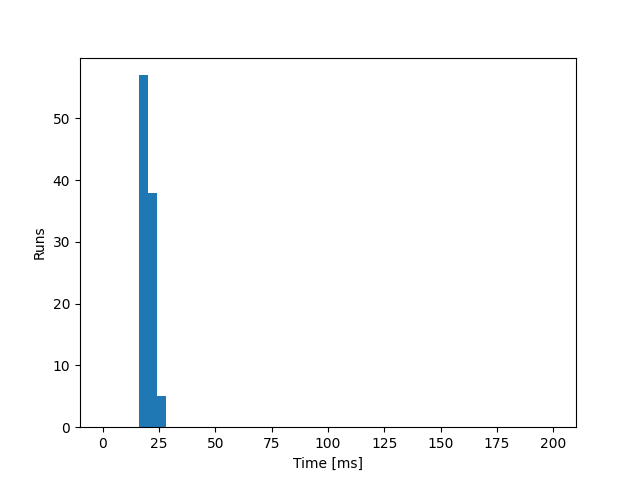
\includegraphics[width=\textwidth]{tests/reading-file-1M.bpf-wasmtime.png}
    \caption{eBPF (1 MB)}
  \end{subfigure}

  \begin{subfigure}[b]{0.32\textwidth}
    \centering
    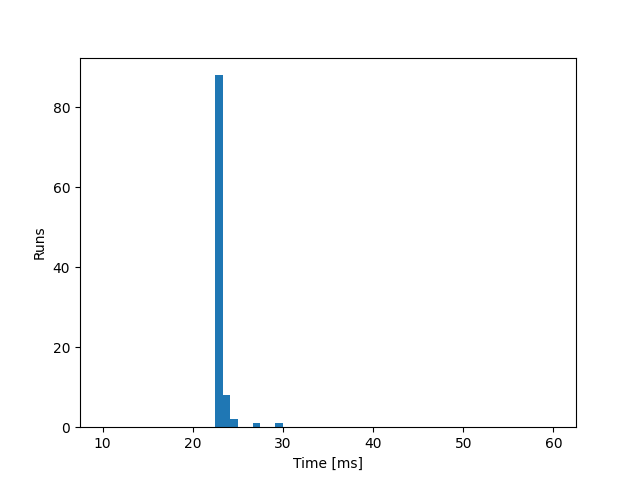
\includegraphics[width=\textwidth]{tests/reading-file-10M.wasmtime.png}
    \caption{Wasmtime (10 MB)}
  \end{subfigure}
  \begin{subfigure}[b]{0.32\textwidth}
    \centering
    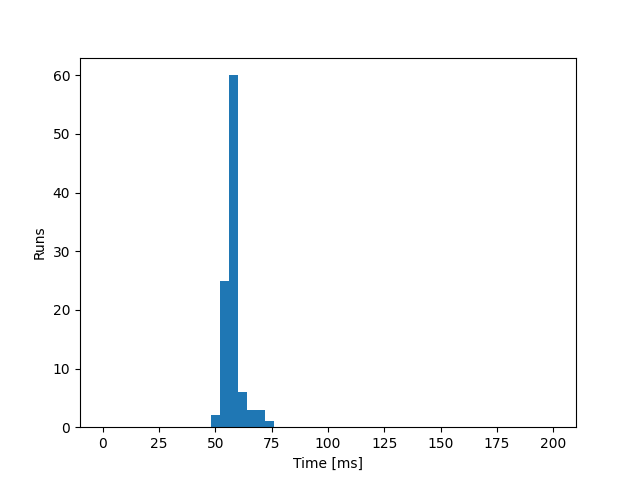
\includegraphics[width=\textwidth]{tests/reading-file-10M.landlock.png}
    \caption{Landlock (10 MB)}
  \end{subfigure}
  \begin{subfigure}[b]{0.32\textwidth}
    \centering
    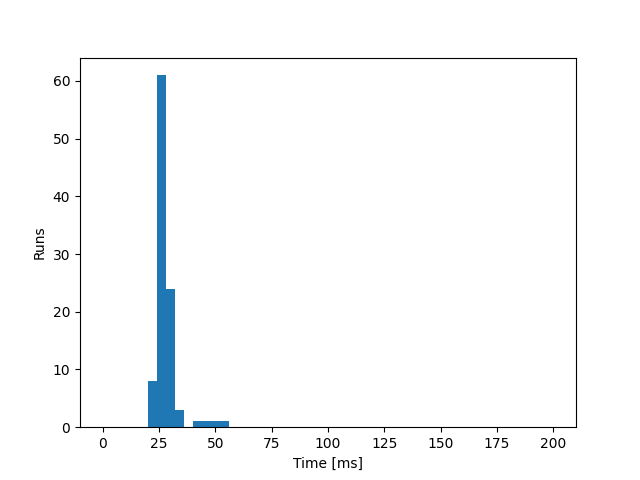
\includegraphics[width=\textwidth]{tests/reading-file-10M.bpf-wasmtime.png}
    \caption{eBPF (10 MB)}
  \end{subfigure}

  \begin{subfigure}[b]{0.32\textwidth}
    \centering
    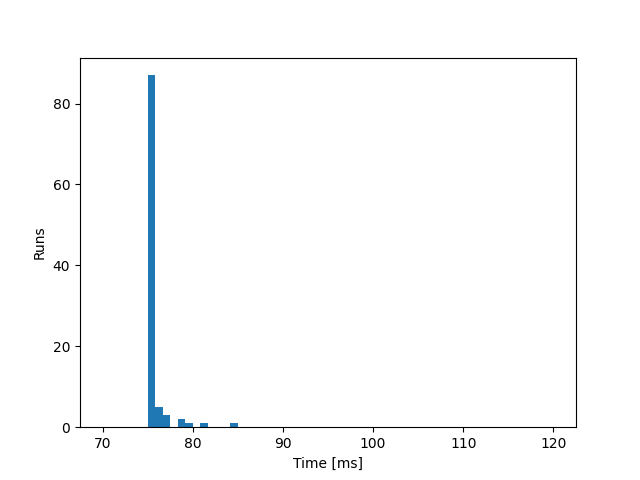
\includegraphics[width=\textwidth]{tests/reading-file-100M.wasmtime.png}
    \caption{Wasmtime (100 MB)}
  \end{subfigure}
  \begin{subfigure}[b]{0.32\textwidth}
    \centering
    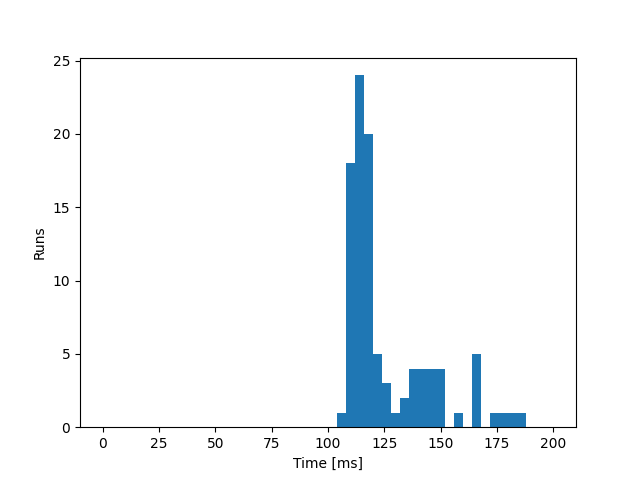
\includegraphics[width=\textwidth]{tests/reading-file-100M.landlock.png}
    \caption{Landlock (100 MB)}
  \end{subfigure}
  \begin{subfigure}[b]{0.32\textwidth}
    \centering
    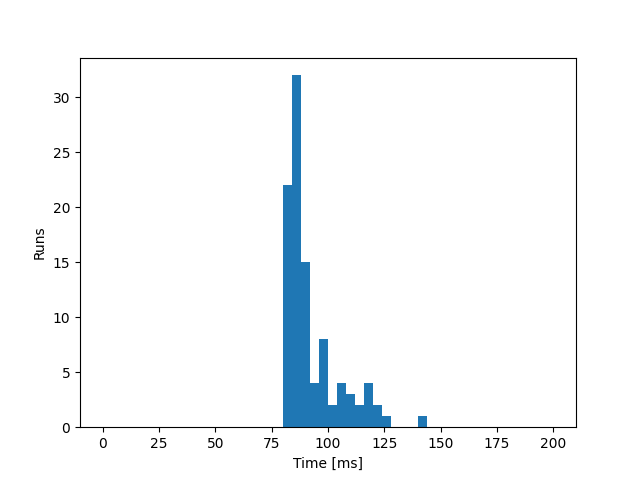
\includegraphics[width=\textwidth]{tests/reading-file-100M.bpf-wasmtime.png}
    \caption{eBPF (100 MB)}
  \end{subfigure}

  \caption{Distribution of a WASM binary execution times when reading a file.}
  \label{fig:distribution-reading-wasm}
\end{figure}

\section{Internal analysis of the developed project}

\subsection{Performance impact of Landlock}

\subsection{Performance impact of using a WASI library}

\section{Conclusions and observations}